In this stage, the classifier and the regressor have been implemented after preparing the data in specified format. Weka's library file has been used in Java programming language to implement the algorithms and train the models based on the curated data.
Following are the sample snippets of parts of data and algorithms used thus far:-
\begin{itemize} 
\item{Dataset: Our data is in arff format. The columns in the data are as given below:}

\begin{itemize}
\item{Day of Month:}
This nominal attribute takes values ranging from 1 to 3 and captures the relation between time delay and time of the month.
\item{Day of week:}
This nominal attribute takes values ranging from 1 to 7 and captures the relation between time delay and day of the week to learn differences in weekdays and weekends.
\item{Origin:}
This nominal attribute indicates the origin airport for the departing flight. Its values are indicated by three letter abbreviation for the airport name.
\item{Carrier:}
This nominal attribute tries to include relation between a particular flight carrier and the delay in its flights. Its values are denoted by wo letter abbreviation of the flight carrier name.
\item{Departure Time:}
This nominal attribute indicates what time of the day the flight is departing. It can either be 0(morning), 1(afternoon) or 2(night).
\item{Dep Delay New:}
This attribute indicates by how many minutes the flight has been delayed. It is of numeric type. It acts as the response variable for our regressor model.
\item{Dep Delay 15:}
This nominal attribute acts as our class variable for the classifier. If delay in flight departure is more than 15 minutes, it is classified as delayed, otherwise as not delayed.
\item{Distance:}
This nominal attribute with values ranging from 0 to 10 indicates distance the flight has to travel. We know that departure delay for a flight has little to do with the distance the flight has to travel, so we included this attribute to test the significance for the same in our models.
\item{Sample data: Order is as shown above:}
\\1 , 2 , LAX , AA , 1 , 32 , 1 , 9\\
3 , 6 , ORD , F9 , 2 , 22 , 1 , 6\\
4 , 4 , JFK , EV , 2 , 9 , 0 , 6\\
30 , 3 , EWR , WN , 1 , 144 , 1 , 4\\
30 , 3 , EWR , WN , 2 , 62 , 1 , 3
\end{itemize}
\item{Output: The sample outputs of the classifier and the regressor for training and testing sets are as follows:}
\begin{itemize}
\item{Naive Bayes Tree Classifier:}
\\\\---Build Tree---\\
tree size:12\\
leaf size:9\\
\% correct: 85.80\\
\\---Test Data---\\
Input: 11,5,B6,JFK,0,4\\
class:notdelayed classified as:notdelayed\\
Input: 9,3,OO,LAX,1,1\\
class:delayed classified as:delayed\\
Input: 22,2,AA,ORD,1,6\\
class:notdelayed classified as:delayed\\
\% correct: 66.67\\
\item{J48 Classifier:}
\\\\---Build Tree---\\
tree size:208\\
leaf size:142\\
\% correct: 86.39\\
\\---Test Data---\\
Input: 1,2,AA,LAX,1,9,32\\
class:delayed  classified as:delayed\\
Input: 1,2,AA,ORD,2,6,22\\
class:delayed  classified as:delayed\\
Input: 1,2,AA,JFK,2,6,29\\
class:notdelayed classified as:notdelayed\\
\% correct: 100.0\\
\item{Random Forest Classifier:}
\\\\---Random Forest---\\
Random forest of 100 trees, each constructed while considering 3 random features.\\
Out of bag error: 0.1515\\
\% correct: 84.41\\
\\---Test Data---\\
Input: 8,3,F9,EWR,0,3\\
class:notdelayed classified as:delayed\\
Input: 11,1,WN,LAX,1,1\\
class:delayed classified as:delayed\\
Input: 29,6,AA,ORD,1,5\\
class:notdelayed classified as:delayed\\
\% correct: 33.34\\
\item{Rule based Classifier:}
\\\\---Decision Table---\\
Number of Rules : 1218\\
\% correct: 86.29\\
\item{Simple Naive Bayes Classifier:}
\\\\---Naive Bayes---\\
\% correct: 85.75\\

\item{Sample decision tree:}\\
Consider a sample decision tree for two attributes, origin and day of month. The classes will be "delayed" and  "not delayed". As shown in Fig 3, following is a sample decision tree generated by the classifier:\\


$ORIGIN\\
ORIGIN=LAX\\
|DAYOFMONTH\\
||DAYOFMONTH<15\{delayed\}\\
||DAYOFMONTH>=15\{not\ delayed\}\\
ORIGIN=JFK\\
|DAYOFMONTH\\
||DAYOFMONTH<15\{not\ delayed\}\\
||DAYOFMONTH>=15\{delayed\}\\
$
\begin{figure}
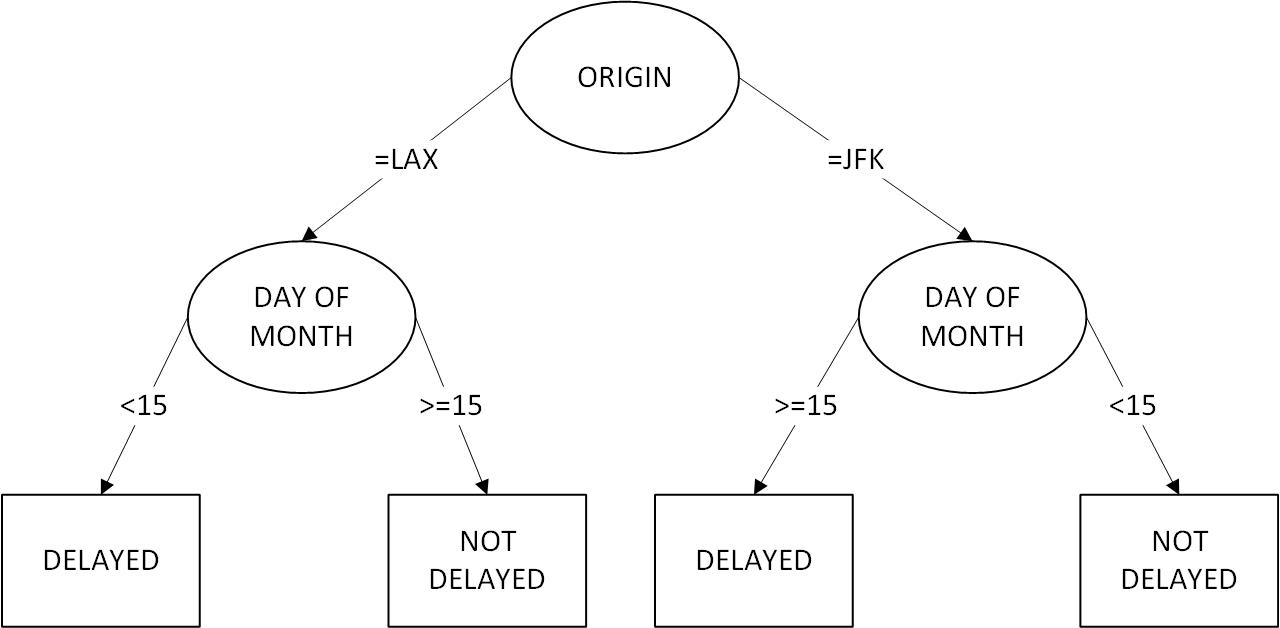
\includegraphics[width=\linewidth]{decisiontree.jpg}
\caption{Sample decision tree for 2 attributes}
\end{figure}

\item{Multiple Linear Regression:}\\
\\---MLM equation---\\
DEPDELAYNEW =\\ 4.2139 *  DAYOFMONTH=26,23,30,12,25,\\
27,24,20,15,28,21,2,14,7,3,18,4,17,10,8 +\\
3.7402 * DAYOFMONTH=15,28,21,2,14,\\
7,3,18,4,17,10,8 +\\
4.9167 * DAYOFMONTH=18,4,17,10,8 +\\
3.503  * DAYOFMONTH=17,10,8 +\\
6.7863 * DAYOFMONTH=8 +\\
7.2751 * CARRIER=MQ,B6,AA,DL,OO,EV,UA +\\
3.4147 * CARRIER=AA,DL,OO,EV,UA +\\
5.0166 * CARRIER=EV,UA +\\
5.03 * ORIGIN=DEN,LAX,JFK,EWR,BOS,ORD +\\
-3.6498 * ORIGIN=EWR,BOS,ORD +\\
5.4878 * ORIGIN=BOS,ORD +\\
9.5943 * DEPTIME=0,2 +\\
26.2807\\
Correlation Coefficient: 0.1919\\\\
---Test Data---\\
Input: 1,2,AA,LAX,1,9,32\\
delay:32.0 predicted delay:41.99\\
Input: 1,2,AA,ORD,2,6,22\\
delay:22.0 predicted delay:53.43\\
Input: 1,2,AA,JFK,2,6,29\\
delay:29.0 predicted delay:51.59\\
\% nearby values: 33.34\%
\end{itemize}

\item{Working code:}
\begin{itemize}
\item{Classifier:}
The classifier class is utilized to build the classification model. The sample code for a J48 classifier in Java to predict class of first instance of the training data is as shown below:-\\
$J48\ j48tree = new\ J48();\\
String\ classes[] = \{ "notdelayed", "delayed" \};\\
DataSource\ data = new\ DataSource("j48train.arff");\\
Instances\ instances = data.getDataSet();\\
int classindex=instances.numAttributes() - 1;\\
instances.setClassIndex(classindex);\\
j48tree.buildClassifier(instances);\\
double \ predictedclass=j48tree.classifyInstance(instances.instance(1));\\
System.out.println(classes[(int)predictedclass]);$



\item{Regressor:}
The regression class is utilized to build the multiple linear regression model. The code for this class in Java to predict delay in flight departure time in minutes is as shown below:-\\
$LinearRegression\ reg = new\ LinearRegression();\\
DataSource\ data = new\ DataSource("regtrain.arff");\\
Instances\ instances = data.getDataSet();\\
int\ classindex=instances.numAttributes() - 1;\\
instances.setClassIndex(classindex);\\
reg.buildClassifier(instances);\\
double\ predicteddelay = reg.classifyInstance(instances.instance(1));\\
System.out.println(predicteddelay);\\
$

\end{itemize}

\item{Demo and sample findings: Here are the observations from running these algorithms on the data:}
\begin{itemize} 
\item{Classifier:}
	For the given data, the J48 algorithm creates a decision tree model with 142 leaf nodes and a total tree size of 208 nodes. It gives an accuracy of 86.39\% on the training data as compared to NBTree which gives 85.80\% accuracy. As for other classification models like Decision Table, Naive Bayes and Random Forest, the accuracy of prediction on test data is less than that of J48 classifier. Thus, we use the J48 decision tree for our classifier model and for the given data attributes, we can say it works pretty well for predicting if a flight will be delayed or not. As for time complexity of classifying a given instance in our data, it will take constant time equal to the height of our decision tree generated. \\
\begin{center}
\begin{tabular}{| l | l | l |}
    \hline
    Algorithm & Model base & Accuracy \\ \hline
    J48 & Tree & 86.39\% \\ \hline
    DecisionTable & Rules & 86.29\% \\ \hline
	NBTree & Tree & 85.80\% \\ \hline
	Naive Bayes & Bayes & 85.75\% \\ \hline
	RandomForest & Forest & 84.41\% \\ \hline
    \end{tabular}
\end{center}
    \ \\Some observations made about the attributes from the j48 decision tree model:-
    \begin{itemize}
    \item{The attribute Departure time is the topmost node in our decision tree. This means that this attribute has the highest effect on delay of a flight, which makes sense as well.   }
    \item{Next, we have the day of month, origin and carrier following with their effect on delay in decreasing order.  }
    \item{Surprisingly, day of week does not have much of an effect on the delay as was previously expected.}
    \end{itemize}
\item{Regressor:}
	The multiple linear regressor model generated from the given data set has a low correlation coefficient. We say the predicted delay is a good enough estimate if it is within 10 minutes of the actual delay in minutes. The given attributes can provide a rough estimate of this delay but in real, there are many more attributes required in order to accurately predict flight departure delay in minutes. Hence, this model is only as good as the attributes present in the data set that can explain the delay in departure time of a flight.\\
    Some observations made about the attributes from the regression model:-
    \begin{itemize}
    \item{The correlation coefficient value of the model is 0.1919 which means there is some relation between the chosen explanatory variables and the response variable delay in flight but the explanatory variables are not sufficient to explain the change in response variable totally.}
    \item{Departure time has a high coefficient in the linear model which means it has a good amount of statistical influence on the delay in flight. This is consistent with our classification model.}
    \item{Other attributes like day of month, carrier and origin airport also have significant value of their coefficients. Again, this is consistent with out classification model.}
	\end{itemize}    
\end{itemize}
\end{itemize}

